\documentclass[11pt,a4paper]{article}
\usepackage[T1]{fontenc}
\usepackage[utf8]{inputenc}
\usepackage{lmodern}
\usepackage[margin=27mm]{geometry}
\usepackage{amsmath,amssymb,amsthm,mathtools,bm}
\usepackage{graphicx,booktabs,longtable,array,tabularx}
\usepackage{float}
\usepackage[numbers,sort&compress]{natbib}
\usepackage{xcolor,hyperref,microtype}
\hypersetup{colorlinks=true,linkcolor=blue!45!black,citecolor=blue!45!black,urlcolor=blue!45!black}
\setlength{\emergencystretch}{2em}
\setlength{\parskip}{0.25em}
\newtheorem{theorem}{Theorem}[section]
\newtheorem{proposition}[theorem]{Proposition}
\newtheorem{lemma}[theorem]{Lemma}
\newtheorem{corollary}[theorem]{Corollary}
\theoremstyle{definition}
\newtheorem{definition}[theorem]{Definition}
\newtheorem{condition}[theorem]{Condition}
\theoremstyle{remark}
\newtheorem{remark}[theorem]{Remark}
\newcommand{\e}{\mathrm e}
\newcommand{\ii}{\mathrm i}
\newcommand{\1}{\mathbf 1}
\newcommand{\CC}{\mathbb C}
\newcommand{\RR}{\mathbb R}
\newcommand{\ZZ}{\mathbb Z}
\newcommand{\QQ}{\mathcal Q}
\newcommand{\Cx}{\mathfrak C_x}
\newcommand{\ip}[2]{\langle #1,#2\rangle}
\newcommand{\norm}[1]{\left\|#1\right\|_2}
\DeclareMathOperator{\diag}{diag}
\DeclareMathOperator{\rank}{rank}
\DeclareMathOperator{\tr}{tr}
\DeclareMathOperator{\Ran}{Ran}

\title{A Seven-Island Framework for Twin-Prime Research:\\
Exact Structures, Analytic Obstructions,\\and Two Bridging Problems}
\author{}
\date{12 September 2026\\English synthesis draft v0.2}
\begin{document}
\pagestyle{plain}
\maketitle
\begin{abstract}
Exact representations of prime-pair problems become useful only when estimates retain the original arithmetic coefficients, scales, and quantifiers. We synthesize a fixed-shift research program around this requirement, using a seven-island map to distinguish objects from the transfers between them. For the prescribed arithmetic operator at interval scale $x$ and prime-modulus scale $Q=x^{1/3}$, we give its exact positive-form decomposition and uniform row-energy bounds. Actual coefficient costs prevent coefficient-blind norm estimates, including ordinary row normalization, from supplying a fixed-power saving. A separate low-frequency argument produces $(1/4+o(1))Q^2$ negative directions, obstructing specified low-rank norm repairs. An exact Kloosterman representation identifies the unproved two-sided attachment needed to exploit a critical-range bilinear estimate. In contrast, an explicit smooth partition already bounds the collective boundary contribution by $xQ^2x^{-11/64+o(1)}$. For the actual moving sieve events, a Chinese-remainder and Abel-summation argument yields variance $O(N)$ and Haar-almost-everywhere infinite recurrence, but not recurrence at the arithmetic seed $0$. The analytic route thus lacks a coefficient-sensitive signed estimate, while the dynamical route lacks a distinguished-point conclusion. We restate and prove selected archived results, clarify their dependencies and conditional loss budgets, and distinguish them from the unresolved twin-prime endpoint. This paper does not prove the twin-prime conjecture.

\end{abstract}
\noindent\textbf{Keywords:} twin primes; M\"obius correlations; reduced residue classes; Gram operators; Kloosterman sums; distinguished seeds.
\clearpage
\setcounter{tocdepth}{1}
\tableofcontents
\medskip
\noindent\textbf{Principal notation and distinct counting objects.}
\begin{center}\small
\begin{tabularx}{\linewidth}{@{}p{.24\linewidth}X@{}}
\toprule
Notation & Meaning and scope\\\midrule
$\pi_2(y),\ S_2(y)$ & Prime-pair count and von Mangoldt pair sum; Section~\ref{sec:arithmetic}.\\
$I_x,\ Q,\ H,\ U$ & Actual interval, prime-modulus scale, kernel scale, and divisor cutoff; Section~\ref{sec:operator}.\\
$\beta,\ w,\ A$ & Prescribed real coefficient vectors and a possibly complex Hermitian matrix.\\
$\Cx=\ip w{A\beta}$ & Mixed off-diagonal scalar; not a prime-pair count.\\
$S_x^{\rm phys}$ & Auxiliary same-index scalar $\sum_{t\in I_x}\beta(t)w(t)$; Section~\ref{sec:bridges}.\\
$S_N,\ A_N,\ Q_N$ & Moving-target hit count, its Haar mean, and sieve primorial; Section~\ref{sec:dynamics}.\\
$A_*,\ E_*,\ K_*$ & Imported folding scalar, error, and terminal divisor; $A_*$ is not the matrix $A$.\\
\bottomrule
\end{tabularx}
\end{center}
\noindent The norm $\|\cdot\|_2$ is Euclidean for vectors and induced for matrices unless a different inner product is stated. The analytic interval size $N=|I_x|$ and the dynamical time $N$ are local to their respective sections.

\clearpage
\section{Introduction: exact structure and arithmetic return}
The twin-prime problem asks for infinitely many prime pairs at the fixed displacement $2$. A recurring difficulty in approaches to this problem is not the absence of useful representations, but the passage from a representation to an estimate for the original arithmetic data. An exact change of variables may preserve every coefficient without producing cancellation. A small normalized matrix may carry large coefficient costs. A full-measure recurrence theorem may omit the one initial point that encodes the integers. These are different gaps, and identifying their mathematical content is the organizing purpose of this article.

We use the seven-island map in Figure~\ref{fig:map} to separate arithmetic foundations, analytic cancellation, fixed atoms, actual occurrences, moving-target dynamics, the twin-prime endpoint, and auxiliary geometric lifts. The islands are not successive steps of a proved implication. We reconstruct selected results by their dependencies, rather than by the order of the archived investigations. The contribution is a source-traceable synthesis with explicit proofs and transfer requirements, not a claim of first discovery or an exhaustive account of every route to twin primes.

\subsection{Two gaps, with different endpoint connections}
The analytic core concerns a specific mixed scalar $\Cx=\ip w{A\beta}$, of natural scale $xQ^2$. The vectors, unit masks, physical interval, Fourier convention, and deleted diagonal are part of its definition. A full-scalar saving with exponent strictly greater than $1/400$ would be useful in the imported analytic interface, but that interface also requires a separate full-shell estimate called Gate A. Both gates lie inside map Bridge A. Their conditional output in this paper is a bound for another auxiliary scalar, $S_x^{\rm phys}$; the complete upstream implication to prime-pair counting is not reproved here.

The dynamical connection is pointwise and explicit: the moving sieve events at seed $0$ identify the pairs $n,n+2$ that are both prime. Adequate mass and covariance control do prove infinite recurrence for almost every seed. They do not establish that the prescribed seed belongs to that good set. Map Bridge B names this return to the distinguished arithmetic point. An auxiliary geometric representation must preserve the same event and seed correspondence; changing the ambient space alone cannot close the gap.

\subsection{Results and their roles}
The main results serve distinct roles. Proposition~\ref{prop:decomp} identifies the exact positive-form structure behind the actual operator. Theorem~\ref{thm:normbarrier}, Corollary~\ref{cor:normalized}, and Theorem~\ref{thm:rank} delimit coefficient-blind norm bounds and low-rank repairs. Proposition~\ref{prop:emitter} identifies the complete Kloosterman arrays, whereas Condition~\ref{cond:compression} states an unproved, loss-controlled attachment to a two-sided short-array estimate. Theorem~\ref{thm:boundary} supplies a genuine bound for one component of the original scalar. Finally, Theorem~\ref{thm:haar} proves metric recurrence for the actual moving targets, and Proposition~\ref{prop:seed} isolates a sufficient, still-unverified way to reach seed $0$.

The distinction between these roles matters. A method obstruction is not a lower bound for the actual scalar. A boundary estimate is not an interior estimate. A sufficient criterion is not a verified hypothesis. In particular, the fixed-atom and occurrence interfaces in Section~\ref{sec:structure} explain what an arithmetic attachment must preserve; they do not construct all the upstream attachments needed by the analytic program.

\subsection{Mathematical inputs and scope}
Our prime-counting input is the classical prime number theorem and its partial-summation consequences~\cite{selberg1949}. The hybrid coefficient's second-moment estimate uses the unconditional Mertens product baseline stated at the beginning of~\cite{lamzouri2015}; none of that paper's conditional bias-distribution results is used. Frequency separation, positive-semidefinite compression, finite Fourier orthogonality, and spectral min--max arguments provide the structural tools.

The critical-interval bilinear estimate of Blomer--Pascadi~\cite{blomer2026} supplies an external benchmark. Its square-root-length specialization offers a local Kloosterman saving under specified support and coprimality conditions. Our question is whether the actual signed expression can be attached to those inputs with all losses paid. The external theorem does not itself provide that attachment.

The source-linked research wiki helped organize the distinctions between definitions, estimates, obstructions, and conditional transfers. It is a secondary reading aid, not independent evidence for a theorem. The original proofs remain the mathematical sources; Appendix~\ref{sec:provenance} and the companion concordance explain how to locate them. A systematic external literature comparison and novelty assessment remain necessary before submission.

\subsection{Reading guide}
Section~\ref{sec:arithmetic} fixes the endpoint and the transfer requirements. Section~\ref{sec:structure} distinguishes literal atom identities, occurrence conservation, and weighted-cover costs. Sections~\ref{sec:operator}--\ref{sec:boundary} develop the analytic results on one common object. Section~\ref{sec:dynamics} treats the metric theorem, seed criterion, and geometric limitations. Section~\ref{sec:bridges} puts the remaining analytic and dynamical obligations side by side. Readers can follow either branch without reading the historical manuscripts in sequence; exact source locations and material not selected here remain in the source matrix and full catalog.

\clearpage
\begin{figure}[p]
\centering
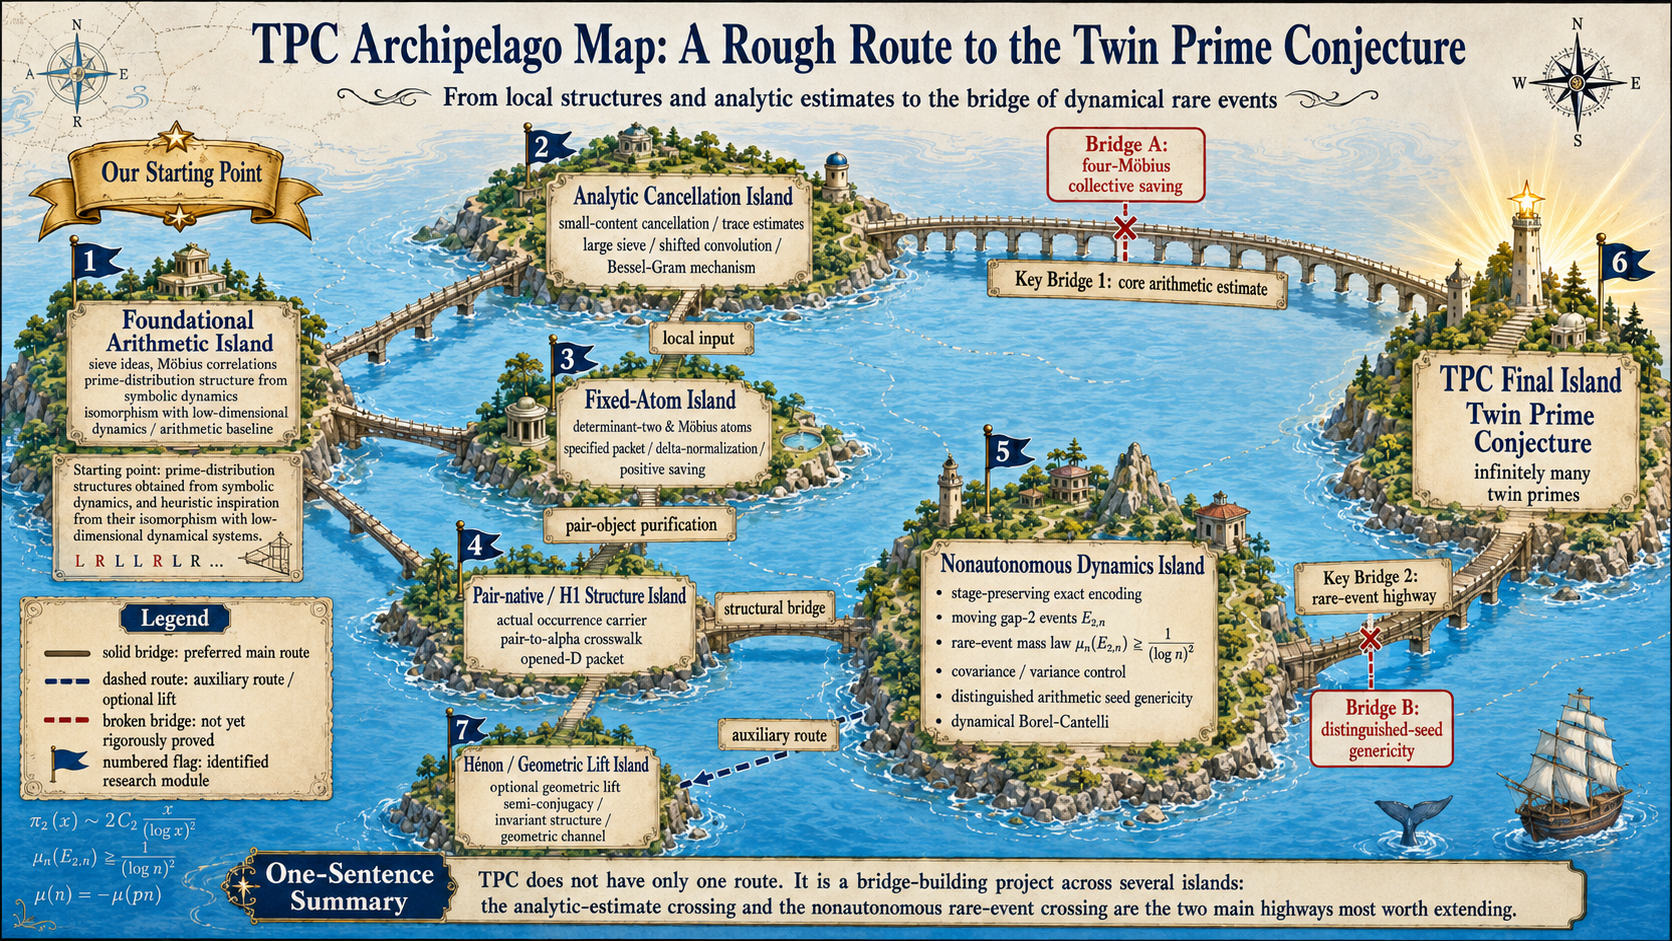
\includegraphics[width=\textwidth]{figures/tpc_route_en.png}
\caption{The user's seven-island map, reproduced unchanged. Islands name objects and tasks, not completed steps. Connections are proposed routes, not certified implications; broken bridges mark unproved transfers, not universal impossibility. Schematic formulae do not establish isomorphisms, savings, or prime-pair asymptotics: the hypotheses in the text govern those claims. Map Bridge A contains both analytic Gate A and Gate B; map Bridge B concerns the distinguished arithmetic seed. Rare-event mass alone does not establish recurrence at that seed. The full-resolution companion preserves the small labels for enlargement.}
\label{fig:map}
\end{figure}
\clearpage

\section{Arithmetic foundations and the endpoint}\label{sec:arithmetic}
\subsection{The endpoint and auxiliary quantities}
Write $\pi_2(y)=\#\{p\le y:p,p+2\text{ are both prime}\}$. The endpoint is $\pi_2(y)\to\infty$, not the discovery of more pairs in a finite interval. A customary weighted auxiliary quantity is
\[
S_2(y)=\sum_{n\le y}\Lambda(n)\Lambda(n+2),
\]
where $\Lambda$ denotes the von Mangoldt function. An asymptotic such as $S_2(y)\sim cy$ with $c>0$ would imply infinitely many twin primes. This is a sufficient condition, not an asymptotic proved here.

To justify the implication, one must remove proper prime powers. There are $O(\sqrt y\log y)$ pairs in which at least one coordinate is $p^k$ with $k\ge2$, and each weight is $O(\log^2y)$. Their total contribution is $o(y)$. Finitely many genuine prime pairs cannot account for a positive linear main term. Even for a standard auxiliary quantity, its connection to the endpoint should therefore be stated rather than inferred from its name.

\subsection{Island 1: local sieve factors versus prime-pair counts}
For $y\ge2$, put $P_y=\prod_{p\le y}p$, $s_y(n)=\1_{(n,P_y)=1}$, and $\rho_y=\prod_{p\le y}(1-1/p)$. Let $\mathcal H=\{h_1,\ldots,h_r\}\subset\ZZ$ be a fixed finite nonempty set of distinct shifts, and let $\nu_p(\mathcal H)$ count its distinct residues modulo $p$. The Chinese remainder theorem (CRT) gives
\[
C_y(\mathcal H):=\frac1{P_y}\sum_{n\bmod P_y}\prod_{h\in\mathcal H}s_y(n+h)
=\prod_{p\le y}\left(1-\frac{\nu_p(\mathcal H)}p\right).
\]
Indeed, there are $p-\nu_p(\mathcal H)$ allowed classes at each prime, and CRT multiplies these counts. If $\mathcal H$ is admissible, meaning $\nu_p<p$ for every prime, then $\nu_p=r$ for all sufficiently large $p$. The normalized factor is $(1-r/p)(1-1/p)^{-r}=1+O_r(p^{-2})$, so the product converges. In particular,
\[
\frac{C_y(\{0,2\})}{\rho_y^2}\longrightarrow2C_2,\qquad
C_2=\prod_{p>2}\frac{p(p-2)}{(p-1)^2}>0.
\]
This is a classical local calculation, not a new prime-pair asymptotic~\cite{archive1}.

Translate $\min\mathcal H$ to zero, set $h_{\max}=\max\mathcal H$, and let $X\to\infty$. If $Y_X=\sqrt{X+h_{\max}}$ and $Y_X<n\le X$, then every $n+h$ exceeds $Y_X$ and is at most $Y_X^2$. These integers survive the sieve through $Y_X$ if and only if they are all prime. This is a pointwise identification, not an estimate for the number of survivors. By contrast, complete-period decomposition on $1\le n\le X$ only gives
\[
\left|\sum_{1\le n\le X}\prod_{h\in\mathcal H}s_y(n+h)-XC_y(\mathcal H)\right|\le P_y+1.
\]
Complete periods contribute exactly; the remaining partial period costs at most $P_y$, with an additional $1$ for a noninteger endpoint. If $P_y=o(X\rho_y^r)$, this bound makes the normalized error vanish. At the primality-exact cutoff, however, the prime number theorem gives $\log P_{Y_X}\sim\sqrt X$, so this error bound provides no useful relative control. This is a mismatch between two elementary arguments, not an impossibility theorem for all sieve methods.

\subsection{The seven islands are not a serial proof}
\begin{table}[H]
\centering\small
\caption{Division of mathematical tasks. The final column does not assert necessary conditions for every possible route.}
\begin{tabularx}{\textwidth}{c p{.25\textwidth} X}
\toprule
Island & Object or task & Transfer still requiring identification in this framework\\\midrule
1 & Arithmetic foundations & Preserve the original counting interpretation when starting from sieves, correlations, or encodings.\\
2 & Analytic cancellation & Pass from local structure to a signed saving for the complete actual coefficients.\\
3 & Fixed atoms & Control the specified shift, phase, and packet pointwise.\\
4 & Actual occurrences / H1 & Supply complete carriers, source correspondences, multiplicities, and coefficientwise conservation.\\
5 & Nonautonomous dynamics & Pass from a measure statement to recurrence at the specified arithmetic seed.\\
6 & Twin-prime endpoint & Obtain infinitely many genuine prime pairs, not a model statement or finite certificate.\\
7 & Auxiliary geometric lifts & Preserve time and event readout, without assuming arithmetic genericity for free.\\
\bottomrule
\end{tabularx}
\end{table}

\subsection{What every transfer must retain}
To compare expressions from different stages, we record a source specification as
\[
\begin{split}
\mathcal O=(&\text{coefficients},h_0,\text{support and order},\text{parameter range},\\
&\text{quantifiers},\text{normalization},\text{loss budget}).
\end{split}
\]
This is bookkeeping against misapplication, not a new mathematical object. Similar notation does not imply equal specifications. An arbitrarily large CRT origin is not an origin in the prescribed physical interval; a prefix of a full prime shell is not an arbitrary prime selection; recomputing local row energy is not compressing the original normalized matrix.

We distinguish four evidence types: finite identities verified by expansion; uniform propositions with complete hypotheses and proofs; conditional consequences retaining their unproved premises; and finite numerical diagnostics. Diagnostics do not carry infinite quantifiers, and a successful program check does not make a conditional implication unconditional. The results below should be read in this hierarchy, not by their order of appearance in the archive.

\section{Fixed atoms and actual occurrences}\label{sec:structure}
This layer separates three tasks: identifying a retained atom, reconstructing its literal coefficient from children, and covering the actual occurrence vector with estimable blocks. A fixed displacement, phase, modulus, and support are distinct requirements. The identities below are useful only after their source data have been supplied; none constructs the missing production pair-to-atom attachment. A carrier means the indexing set of terms or occurrences, with their source data. The label H1 is inherited from the source program; it does not name an additional result proved here.

\subsection{The order-preserving determinant-two pullback}
Let $I$ be an integer interval, $a,s$ positive integers, and $d,u$ integers satisfying
\[
\begin{gathered}
D(z)=d+sz>0,\quad V(z)=u+az>0\quad(z\in I),\quad su-ad=2,\\
(a,s)=1,\quad(as,2)=1,\quad(d,s)=(u,a)=1.
\end{gathered}
\]
Write $\lambda$ for the Liouville function, distinct from the truncated projector weight below. Let $B,\tau$ be the specified integers and $\chi,W_X$ the functions prescribed by the original block. Its literal coefficient is
\[
a_{\xi,X}(z)=\mu(D(z))\mu(V(z))\1_{(B,V(z))=1}\chi(\tau+Bz)W_X(\tau+Bz).
\]
\begin{proposition}[Exact masked pullback]\label{prop:pullback}
Set $q_{\rm prog}=as$ and $n(z)=su+as z=sV(z)=aD(z)+2$. This is an order-preserving bijection from $I$ onto its image $\mathcal N_I$, and
\begin{align*}
\mu(D(z))\mu(V(z))&=\lambda(q_{\rm prog})\lambda(n-2)\lambda(n)\mathcal Q_{a,s}(n),\\
\mathcal Q_{a,s}(n)&=\mu^2((n-2)/a)\mu^2(n/s).
\end{align*}
For every $\alpha\in\RR$, the original sum is therefore exactly
\[
\sum_{z\in I}a_{\xi,X}(z)\e(-\alpha z)
=\lambda(q_{\rm prog})\sum_{n\in\mathcal N_I}
\lambda(n-2)\lambda(n)\mathcal Q_{a,s}(n)\mathcal W_{\xi,X}(n)\e(-\alpha z(n)),
\]
where $\mathcal W_{\xi,X}(n)=\1_{(B,n/s)=1}\chi(\tau+Bz(n))W_X(\tau+Bz(n))$. The same identity holds for every initial prefix.
\end{proposition}
\begin{proof}
The positivity of $as$ gives order preservation, and $su-ad=2$ gives the two integer quotients. Since $\mu(m)=\mu^2(m)\lambda(m)$ and $\lambda$ is completely multiplicative,
$\lambda(n-2)\lambda(n)=\lambda(a)\lambda(s)\lambda(D(z))\lambda(V(z))$.
Multiplying by $\lambda(as)$, whose square is $1$, proves the coefficient identity. Substitute all remaining factors unchanged, without taking absolute values or removing the quotient-squarefree masks. The increasing bijection maps each initial prefix to its corresponding prefix.
\end{proof}
This is the core interface of TPC127~\cite{archive127}. It also preserves variation along consecutive image points and absolute comparison mass, but does not estimate either quantity. Fixing $h_0=2$ neither fixes one phase across scales nor permits the quotient-squarefree conditions to be discarded.

\subsection{Ordered pairs, child reassembly, and occurrence conservation}
The following examples specify distinct interfaces, not successive completed constructions. The first display illustrates the data that an ordered-pair attachment would have to preserve; its purpose is not to define a new self-contained block estimate.
Squaring a sum produces ordered row pairs, a different carrier from the pair of affine forms above. For example, in the opened-$D$ construction, $N_\alpha(j)=\ell_\alpha d_\alpha j+h_0$, and the off-diagonal coefficient contains
\[
\mu(d_\alpha)\mu(d_\gamma)(\log\ell_\alpha)(\log\ell_\gamma)
r_R(N_\alpha(j))r_R(N_\gamma(j))B_\alpha(j)B_\gamma(j).
\]
Here $r_R$ and $B_\alpha$ denote the truncation factor and row-weight aliases in the source expansion. They are not newly defined free functions, and the display does not attach an actual production pair to an affine atom. The complete TPC18 formula is located in the source matrix. Attachment to a retained atom must still preserve the original joint mask, schedule, and normalization.

For a legitimately retained source term, divisor decomposition gives a useful conservation identity. For $G>0$, set
\[
\lambda_G(v)=\sum_{g\mid v,\ g\le G}\mu(v/g).
\]
Then, for positive integers $d,e$,
\[
\sum_{v\mid(d,e)}\lambda_G(v)=\1_{(d,e)\le G}.
\]
Interchange $g,v$ and use $\sum_{h\mid m}\mu(h)=\1_{m=1}$ to prove the identity. Reconstructing the source requires the weighted sum of all children; one child is not the source coefficient. TPC93's inverse and signed reconstruction hold on its squarefree primitive support. TPC205's composition from production pairs remains conditional on a legitimate attachment~\cite{archivestructure}.

A linear occurrence lift is a separate issue. The source labels $\mathsf{EPS}$, $\mathsf{ETO}$, and $\mathsf{FUM}$ mean eligible-prefix-soft, eligible-tail-open, and frontier-unmapped. The nonsoft domain is
$\mathcal C=\mathcal C^{\mathsf{ETO}}\sqcup\mathcal C^{\mathsf{FUM}}$; retaining only the frontier would omit the eligible tail. If the upstream cut satisfies
\[
\1_{\mathsf{EPS}}^TM^{\mathsf{EPS}}+\1_{\mathcal C}^TM^{\rm ns}=\1_{\mathcal N}^T,
\]
and a supplied lift $L:\CC^{\mathcal C}\to\CC^{\mathcal O}$ satisfies $\1_{\mathcal O}^TL=\1_{\mathcal C}^T$, multiplication gives
\[
\1_{\mathsf{EPS}}^TM^{\mathsf{EPS}}+\1_{\mathcal O}^TLM^{\rm ns}=\1_{\mathcal N}^T.
\]
The sets $\mathcal N,\mathcal C,\mathcal O$ are respectively native terms, nonsoft branches, and retained occurrences with source paths. A retained carrier is not the certified nonzero active support: after inverse aggregation, the literal coefficient must still be certified nonzero. An unevaluated coefficient cannot simply be declared zero. This conditional statement does not construct $L$; row separation, metadata fidelity, and the actual nonzero support must also be supplied. A formal support envelope is not the actual occurrence set.

\subsection{A weighted-cover criterion}
Suppose the actual coefficient vector $c_{\rm phys}$ and admissible-block synthesis matrix $B$ have been supplied, with the specified positive-definite inner products on both spaces. Let $B^\dagger$ be the corresponding Moore--Penrose inverse and $P=BB^\dagger$.
\begin{proposition}[Cover and orthogonal obstruction]
In finite dimensions, the following are equivalent:
\[
c_{\rm phys}\in\operatorname{Ran}B,\qquad Pc_{\rm phys}=c_{\rm phys},\qquad
\langle y,c_{\rm phys}\rangle=0\quad(y\in\ker B^*).
\]
Moreover,
\[
\|(I-P)c_{\rm phys}\|=
\max_{y\in\ker B^*,\ \|y\|\le1}|\langle y,c_{\rm phys}\rangle|.
\]
\end{proposition}
\begin{proof}
The singular value decomposition identifies $P$ as the orthogonal projection onto $\operatorname{Ran}B$, whose orthogonal complement is $\ker B^*$. Orthogonal decomposition gives the equivalences. Cauchy--Schwarz proves the upper bound in the distance formula. A normalized nonzero residual attains equality; when the residual vanishes, both sides are zero.
\end{proof}
This is the linear-algebraic content of the TPC117 criterion~\cite{archivestructure}. Even if $B^\dagger c_{\rm phys}$ gives an exact cover, block bounds $U_b$ still incur the transport cost
$\sum_b|(B^\dagger c_{\rm phys})_b|U_b$.
The existence of a cover is not the existence of an inexpensive cover, much less an arithmetic saving for the actual growing family.

\paragraph{Where this leaves the analytic argument.}
Coefficient conservation, identification of active nonzero occurrences, and a cost-controlled weighted cover are separate requirements. In particular, membership in a union of blocks is weaker than reconstruction of the signed coefficient vector. Section~\ref{sec:operator} therefore starts from its own fully specified source scalar; it is not presented as a consequence of a production lift proved in this section. This keeps a useful structural interface from being mistaken for a completed arithmetic reduction.

\section{The actual operator: definition and exact structure}\label{sec:operator}
Sections~\ref{sec:operator}--\ref{sec:boundary} use one object from the fully recovered scalar specification~\cite{archivev59,archivephysical}. Here ``physical'' means the arithmetic data actually prescribed by the research problem, as opposed to models in which signs, origins, or kernels may be freely selected. We first define that object, then establish its operator structure; subsequent sections distinguish what follows from generic norm information, exact Kloosterman representation, and the small support of the boundary.

\subsection{Parameters, coefficients, and kernel}
Let $x\to\infty$ and set
\[
I_x=(x/2,x]\cap\ZZ,\quad N=\lfloor x\rfloor-\lfloor x/2\rfloor,\quad
Q=x^{1/3},\quad H=x^{21/32},\quad U=x^{133/400}.
\]
The older source scale is $x=2X$, so $N=X+O(1)$. Let $\QQ=\{q\text{ prime}:Q<q\le2Q\}$. Fix $K>0$, put $z=(\log x)^K$, and define
\begin{align}
P(z)&=\prod_{p\le z}p,&W_z&=\prod_{p\le z}\frac p{p-1},&
C_z&=\prod_{p>z}\left(1-\frac1{(p-1)^2}\right),\nonumber\\
b_x^{(z)}(u)&=\1_{I_x}(u)C_zW_z\1_{(u+2,P(z))=1}
\prod_{\substack{p\mid u\\p>z}}\frac{p-1}{p-2},\label{eq:hybrid}\\
\beta(t)&=\frac{\Lambda(t)}{\log t}-\sum_{\substack{d\mid t\\d\le U}}\mu(d),\nonumber\\
w(u)&=\Lambda(u+2)-b_x^{(z)}(u).\label{eq:lanes}
\end{align}
Take $x$ sufficiently large that $z\ge2$. The parameter $K$ is fixed before the threshold is chosen; no assertion is made for growing $K$. The small-prime product includes $2$, and its forbidden residue is $-2$. The symbol $\mu$ in $\beta$ is the M\"obius function. Both actual coefficient vectors are real, but their signs may vary.

Fix a nonnegative real smooth function $\psi_+$ supported in $[-1,1]$ with integral $1$. Write $\e(t)=\exp(2\pi\ii t)$ and
\[
\kappa(y)=\int_{\RR}\psi_+(v)\e(-vy)\,dv,\qquad K_H(h)=\kappa(h/H).
\]
The profile need not be even, so $\kappa$ need not be real. Nevertheless, $\kappa(-y)=\overline{\kappa(y)}$ and $\kappa(0)=1$. The kernel is Schwartz, not identically zero for $|h|>H$. Reflection, $\psi_+(v)=\psi(-v)$, reconciles this convention with the older positive-sign Fourier convention.

\subsection{The complete scalar and row energy}
Set $a_q=q/(q-1)$ and define, on $\ell^2(I_x;\CC)$,
\[
A_q(u,t)=a_q\kappa((u-t)/H)
\big((q-1)\1_{q\mid u-t}-1\big)\1_{q\nmid u}\1_{q\nmid t}\1_{u\ne t},
\qquad A=\sum_{q\in\QQ}A_q.
\]
With $\ip fg=\sum\overline f g$, the target scalar is
\begin{equation}
\Cx=\ip w{A\beta}
=\sum_{q\in\QQ}q\sum_{\substack{u,t\in I_x\\u\ne t,\ q\nmid ut}}
w(u)\beta(t)K_H(u-t)\left(\1_{u\equiv t\ (q)}-\frac1{q-1}\right).
\label{eq:scalar}
\end{equation}
The outer factor $q$ is already present in the matrix definition and must not be inserted twice. The matrix is Hermitian, but its mixed scalar between two real vectors can still be complex.

The row energy under consideration is
\[
G(u)=\sum_{q\in\QQ}\sum_{t\in I_x}|A_q(u,t)|^2,\quad
D_G=\diag(G(u)),\quad Z=D_G^{-1/2}AD_G^{-1/2}.
\]
The square is taken separately at each prime; cross-prime terms are absent. Whenever every $G(u)>0$,
\begin{equation}
\Cx=\ip{D_G^{1/2}w}{Z D_G^{1/2}\beta}.\label{eq:readout}
\end{equation}
A smaller normalized operator norm therefore need not reduce the original scalar: the costs of both weighted vectors must also be counted.

\subsection{The reduced-residue correction}
\begin{proposition}[Exact positive-form decomposition]\label{prop:decomp}
Let $r_q(n)=q\1_{q\mid n}-1$ and define
\begin{align*}
T(u,t)&=\kappa((u-t)/H)\sum_{q\in\QQ}\sum_{a=1}^{q-1}\e(a(u-t)/q),\\
R(u,t)&=\kappa((u-t)/H)\sum_{q\in\QQ}\frac{r_q(u)r_q(t)}{q-1},\\
\Delta(u)&=\sum_{q\in\QQ}a_q(q-2)\1_{q\nmid u}.
\end{align*}
Then $A=T-R-\diag\Delta$ and, in positive-semidefinite order,
\[
R\ge0,\qquad0\le A+\diag\Delta\le T.
\]
\end{proposition}
\begin{proof}
On residues modulo $q$, put
\[
F_q(r,s)=q\1_{r=s}-1,\qquad
S_q(r,s)=a_q\big((q-1)\1_{r=s}-1\big)\1_{r\ne0}\1_{s\ne0}.
\]
When both residues are nonzero, exactly one is zero, or both are zero, respectively, $F_q-S_q$ equals $1/(q-1)$, $-1$, or $q-1$. Hence
\[
F_q-S_q=\frac{r_qr_q^*}{q-1}.
\]
Also, $F_q/q$ projects orthogonally onto the mean-zero subspace of all residues, while $S_q/q$ projects onto the subspace vanishing at zero and summing to zero over the units. Thus $0\le S_q\le F_q$.

Pullback along $I_x\to\ZZ/q\ZZ$ preserves this order and does not require equal residue multiplicities. For the diagonal matrix $D_v(n,n)=\e(-vn/H)$,
\[
[\kappa((u-t)/H)S_q(u,t)]_{u,t\in I_x}
=\int\psi_+(v)D_vS_qD_v^*\,dv.
\]
Integration against a nonnegative weight preserves the order. Sum over primes and remove the exact diagonal $S_q(n,n)=a_q(q-2)\1_{q\nmid n}$ to conclude.
\end{proof}
After diagonal deletion, $A$ need not be positive semidefinite. The negative directions below arise precisely at this stage. Dropping $\Delta$ during reassembly changes the problem.

\section{Norm bounds and coefficient-blind obstructions}\label{sec:barriers}
The next bounds answer a methodological question: can the desired saving follow from the operator norm and coefficient-vector norms alone? The row estimates and actual coefficient norms quantify the cost of that approach. The later rank argument strengthens the obstruction to a particular family of repairs, without identifying the arithmetic vectors with extremizing directions.
\subsection{An upper bound from frequency separation}
Fix finite constants $B_\psi,B_\kappa$ such that
\[
0\le\psi_+(v)\le B_\psi(1+|v|)^{-2},\qquad
|\kappa(y)|\le B_\kappa(1+|y|)^{-2}.
\]
\begin{lemma}\label{lem:upper}
For $Q\ge2$,
\[
\norm A\le4B_\psi(H+4Q^2)+3Q^2.
\]
\end{lemma}
\begin{proof}
Distinct reduced fractions $a/q$ are separated on the circle by at least $(4Q^2)^{-1}$, including the gap across zero. The convolution kernel
$\kappa(h/H)\sum_{q,a}\e(ah/q)$ on all integers has Fourier multiplier
\[
m(\theta)=H\sum_{q,a}\sum_{k\in\ZZ}\psi_+\big(H(a/q-\theta-k)\big)\ge0
\]
by Poisson summation for the fixed Schwartz kernel. The points on the right are separated on the real line by at least $s=H/(4Q^2)$. Each half-open unit interval contains at most $1+1/s$ points. Splitting the positive and negative half-lines and summing $(1+j)^{-2}$ gives
$m(\theta)\le4B_\psi H(1+1/s)$.
Compression to $I_x$ cannot increase the norm. Proposition~\ref{prop:decomp} gives $\norm{A+\diag\Delta}\le\norm T$, and
$\max\Delta<\sum_{Q<q\le2Q}q\le3Q^2$. The claimed bound follows.
\end{proof}
Since $H<Q^2$, the physical scales satisfy $\norm A\ll_\psi Q^2$. No cancellation in $\beta,w$ is used.

\subsection{Energy of every actual row}
\begin{proposition}\label{prop:energy}
For the fixed kernel and every sufficiently large $x$, uniformly in $u\in I_x$,
\[
G(u)\asymp_\psi\frac{HQ^2}{\log Q}.
\]
\end{proposition}
\begin{proof}
Continuity and $\kappa(0)=1$ give fixed $0<\rho,b\le1$ with $|\kappa(y)|\ge b$ for $|y|\le\rho$. For $q\nmid u$, put
\[
S_q(u)=\sum_{\substack{t\in I_x\\t\ne u,\ q\nmid t}}|\kappa((u-t)/H)|^2,\quad
C_q(u)=\sum_{\substack{t\in I_x\\t\ne u,\ q\mid u-t}}|\kappa((u-t)/H)|^2.
\]
Squaring gives the exact identity
\[
G(u)=\sum_{\substack{q\in\QQ\\q\nmid u}}a_q^2
\big(S_q(u)+(q-1)(q-3)C_q(u)\big).
\]
Integral comparison yields $S_q(u)\le2B_\kappa^2H/3$ and
$C_q(u)\le2B_\kappa^2H/(3q)$. Since $1+(q-1)(q-3)/q\le q$, the contribution of each prime is at most $(2B_\kappa^2/3)a_q^2qH$.

If $N-1\ge2\rho H$ and $H\ge2Q/\rho$, at least one side of every row contains
$\lfloor\rho H/q\rfloor\ge\rho H/(2q)$ nonzero congruent differences. Their entries are still units, and $(q-2)^2\ge q^2/9$. This prime therefore contributes at least $(\rho b^2/18)a_q^2qH$.

An integer $u\le x=Q^3$ has at most two distinct prime factors greater than $Q$. Removing the primes dividing $u$ from
$S_Q=\sum_{q\in\QQ}a_q^2q$ loses at most $9Q$. The prime number theorem and partial summation give $S_Q\sim(3/2)Q^2/\log Q$. Beyond a common threshold $S_Q\ge18Q$, so
\[
\frac{\rho b^2}{36}HS_Q\le G(u)\le\frac{2B_\kappa^2}{3}HS_Q
\]
for all actual rows.
\end{proof}
The restriction $u\le Q^3$ is essential to this argument. This is not a theorem for equal-length intervals at arbitrary huge origins or for arbitrary coordinate prefixes.

\subsection{A constant-vector witness and the actual coefficients}
The following lower bounds concern the norm-product upper-bound expression
\[
|\Cx|\le\norm A\,\norm w\,\norm\beta.
\]
They do not give a lower bound for $|\Cx|$.
\begin{theorem}[Obstruction to coefficient-blind norm bounds]\label{thm:normbarrier}
For the fixed data of Section~\ref{sec:operator},
\[
\norm A\ge(3/2+o(1))\frac{Q^2}{\log Q},\qquad
\norm w^2\sim\frac x2\log x,\qquad
\norm\beta^2\ge\left(\frac12\log\frac{27}{22}+o(1)\right)\frac x{\log x}.
\]
Consequently,
\[
\liminf_{x\to\infty}\frac{\log Q}{xQ^2}\norm A\,\norm\beta\,\norm w
\ge\frac34\sqrt{\log(27/22)}>0.
\]
Any proof using only $B_x\norm\beta\norm w$, with $B_x\ge\norm A$, cannot by itself supply a fixed positive power saving.
\end{theorem}
\begin{proof}
Let $f=N^{-1/2}\1_{I_x}$. Before diagonal deletion, the positive form is
\[
\ip f{(A+\diag\Delta)f}=\frac1N\sum_q q\int\psi_+(v)V_q(v/H)\,dv,
\]
where $V_q(\alpha)$ is the sum of squared deviations of the unit-residue sums
$\sum_{n\equiv r(q),\,n\in I_x}\e(\alpha n)$ from their mean over the units. It is not further divided by $q-1$. Write
$I_x=\{a+1,\ldots,a+N\}$ and $N=mq+s$, $0\le s<q$, and define
\[
\begin{gathered}
G_m(y)=\sum_{k=0}^{m-1}\e(ky),\\
S_j(\alpha)=\e(\alpha(a+j))\bigl(G_m(\alpha q)+\1_{j\le s}\e(\alpha mq)\bigr),
\quad1\le j\le q.
\end{gathered}
\]
The sum $S_j$ is exactly the residue sum for $a+j$, comprising $m$ complete periods and at most one terminal term. If $0<|\alpha|q\le1/2$,
\[
|G_m(\alpha q)|\le(2|\alpha|q)^{-1},\qquad
|\e(\alpha j)-1|\le2\pi|\alpha|q\quad(1\le j\le q).
\]
Each sum thus lies within $\pi+1$ of a common center, and within $1$ when $\alpha=0$. Subtracting the mean minimizes the sum of squared distances, giving $V_q(\alpha)\le q(\pi+1)^2$. The fixed frequency support and the eventual inequality $2Q/H<1/2$ place the whole integral in this range. The positive form is therefore
$O(Q^3/(N\log Q))=O(1/\log Q)$.
On the other hand, the number of unit integers is $N_q=N(1-1/q)+O(1)$, whence
\[
\ip f{Af}=-\sum_{q\in\QQ}(q-2)+O(1/\log Q).
\]
The prime number theorem and partial summation give the operator lower bound.

For $w$, define $c(p)=((p-1)/(p-2))^2-1=O(1/p)$ and extend multiplicatively on squarefree integers. Expand the nonnegative Euler product, discard masks bounded by $1$, and enlarge the interval to obtain
\[
\norm{b_x^{(z)}}^2\le xW_z^2\prod_{p>z}(1+c(p)/p)\ll xW_z^2.
\]
The product converges since $c(p)/p=O(p^{-2})$. Mertens' product theorem gives
$W_z\ll\log z\ll_K\log\log x$. The prime number theorem also gives
$\sum_{u\in I_x}\Lambda(u+2)^2\sim(x/2)\log x$, with proper prime powers contributing a lower-order term. The two-sided triangle inequality for norms proves the asymptotic for $w$, without assuming orthogonality between $b_x^{(z)}$ and $\Lambda$.

For $\beta$, take primes $x^{2/5}<p\le x^{9/20}$ and $x/(2p)<r\le x/p$. Eventually $p<r$, and both exceed $U$. Thus $n=pr\in I_x$, $\Lambda(n)=0$, and the only divisor of $n$ at most $U$ is $1$, so $\beta(n)=-1$. The smaller prime factor is unique, avoiding repeated counts. The ordinary prime number theorem in doubling intervals is uniform over this range. The number of such products is
\[
(1+o(1))\frac x2\sum_{x^{2/5}<p\le x^{9/20}}\frac1{p\log(x/p)}
=\left(\frac12\log\frac{27}{22}+o(1)\right)\frac x{\log x}.
\]
The final equality follows by partial summation and
$\int_{2/5}^{9/20}[a(1-a)]^{-1}\,da=\log(27/22)$.
Multiplying the three lower bounds proves the last assertion.
\end{proof}

\begin{corollary}\label{cor:normalized}
For the specified row-energy normalization,
\[
H^{-1}\ll_\psi\norm Z\ll_\psi(\log Q)/H.
\]
Moreover, $\norm Z\,\norm{D_G^{1/2}\beta}\,\norm{D_G^{1/2}w}$ is still at least
$c_\psi xQ^2/\log Q$ for some $c_\psi>0$.
\end{corollary}
\begin{proof}
Since $A=D_G^{1/2}ZD_G^{1/2}$,
$\norm A/G_{\max}\le\norm Z\le\norm A/G_{\min}$.
Each weighted vector contributes a factor of at least $\sqrt{G_{\min}}$ relative to its unweighted norm. Thus the norm-product expression is at least
\[
(G_{\min}/G_{\max})\norm A\norm\beta\norm w.
\]
Apply Proposition~\ref{prop:energy} and Theorem~\ref{thm:normbarrier}.
\end{proof}
This is a lower bound on an upper-bound expression, not a lower bound on $|\Cx|$. It does not rule out cancellation between the actual coefficients, other preconditioners, or coefficient-sensitive methods.

The distinction also explains why the norm upper bound remains useful. In Section~\ref{sec:boundary}, one coefficient vector is restricted to a much smaller boundary support. That support gain pays for a remainder even though the same norm estimate, applied to both full vectors, cannot pay for the desired full-scalar saving.

\subsection{A growing number of negative directions}
The subspaces in the next result witness an operator obstruction; they are not identified with the actual coefficient vectors $\beta,w$.
\begin{theorem}[A scoped obstruction to low-rank repairs]\label{thm:rank}
Put $\tau_x=Q^2/\log Q$ and
\[
J_x=\left\lfloor N\left(\frac1{4Q}-\frac1H\right)\right\rfloor,\qquad
d_x=2J_x+1,\qquad k_x=d_x-35.
\]
For all sufficiently large $x$, there is a complex subspace $W_x$ such that
\[
\dim_\CC W_x\ge k_x,\qquad
\ip f{Af}\le-\frac{\tau_x}{2}\norm f^2\quad(f\in W_x).
\]
Every matrix $E$ of complex rank less than $k_x$, even if non-Hermitian, satisfies
$\norm{A-E}\ge\tau_x/2$, and $k_x=Q^2/4-x^{11/32}+O(1)$.
\end{theorem}
\begin{proof}
Set $U_0=A+\diag\Delta\ge0$ and take $f_j(n)=N^{-1/2}\e(jn/N)$ for $|j|\le J_x$. These vectors are orthonormal on $N$ consecutive integers, and eventually $d_x<N$. For all $q\le2Q$ and $|v|\le1$, we have $q|j/N+v/H|\le1/2$. The preceding residue-variance bound gives
\[
\ip{f_j}{U_0f_j}\le\frac{C_0}{N}\sum_q q^2,\qquad C_0=(\pi+1)^2.
\]
Let $F$ have these vectors as columns, $B=F^*U_0F\ge0$, and $M_1=\sum_q q$. Then
\[
\tr B\le C_0(1+2Q/N)M_1.
\]
An actual integer is divisible by at most two shell primes, so
\[
\Delta(n)\ge D_*:=\sum_q\frac{q(q-2)}{q-1}-4Q\sim\frac32\tau_x.
\]
The number of eigenvalues of $B$ exceeding $D_*/2$ is at most $2\tr B/D_*<35$ eventually, and eventually $D_*\ge\tau_x$. Map the $[0,D_*/2]$ spectral subspace of $B$ through $F$ to obtain $W_x$. At most $35$ dimensions are lost; on this space the $U_0$ form is at most $D_*/2$, whereas the removed diagonal is at least $D_*$. This proves negativity. If $\rank E<k_x$, then $W_x\cap\ker E$ is nonzero. A unit vector in the intersection gives
$\norm{A-E}\ge|\ip f{(A-E)f}|\ge\tau_x/2$.
Finally, expand $d_x$ using $N=x/2+O(1)$ to obtain the dimension asymptotic.
\end{proof}
The spectral cutoff does not say that the whole low-frequency band is negative, or that repairs above some higher rank must succeed.

Real witnesses require a separate construction; a complex spectral space cannot simply be renamed a real one. In the same symmetric band, form the real orthonormal matrix $V$ from
$f_0$, $(f_j+f_{-j})/\sqrt2$, and $(f_j-f_{-j})/(\ii\sqrt2)$.
The real symmetric matrix $\operatorname{Re}(V^*U_0V)$ is positive semidefinite and has trace $\tr B$. Repeating the spectral cutoff gives a different real subspace of dimension at least $k_x$. In particular, for a real-linear map
\[
E:\RR^{I_x}\longrightarrow\CC^{I_x},\qquad\rank_{\RR}E<k_x,
\]
a unit vector in its kernel intersected with this real negative subspace gives
$\|A-E\|_{\RR^{I_x}\to\CC^{I_x}}\ge\tau_x/2$.
The norm uses the Euclidean unit sphere in the real domain, and rank means real image dimension, not complex rank. The identity
$f^TAf=f^T\operatorname{Re}(A)f$ applies to a quadratic form at one real vector. It cannot replace the mixed scalar $w^TA\beta$ by $w^T\operatorname{Re}(A)\beta$.

\section{Kloosterman emission and two-sided attachment}\label{sec:emitter}
The full-range representation and the critical-range estimate concern different inputs. The former retains the exact positive packets and has a saturation identity; the latter acts on two short arrays. The relevant attachment must therefore be made to the signed, diagonal-removed expression, with explicit recombination and residual costs. This section makes that distinction quantitative.
\subsection{The complete Kloosterman representation}
Let $\eta_b$ be the real partition functions constructed in Section~\ref{sec:boundary}, and define the finite set of physical labels
\[
\mathcal J_x=\{j\in\ZZ:\operatorname{supp}\eta_{j,H}\cap[x/2,x]\ne\varnothing\},
\qquad |\mathcal J_x|=O(x/H+1).
\]
All ordered block pairs and their sums in this section are restricted to $(b,c)\in\mathcal J_x^2$. Set
$a^{(j)}(t)=\eta_b(t)\beta(t)+\ii^j\eta_c(t)w(t)$ for $j=0,1,2,3$.
For fixed $q\in\QQ$ and $v\in\RR$, define the sums on unit residue classes and their centered versions by
\[
F_r^{(j)}=\sum_{t\in I_x,\ t\equiv r(q)}a^{(j)}(t)\e(vt/H),\qquad
F_r^{(j),0}=F_r^{(j)}-\frac1{q-1}\sum_{s\ne0}F_s^{(j)}.
\]
Set the centered vector to zero at the zero residue class. Suppressing the superscript $j$, put
\[
\alpha_m=\frac1q\sum_{r\ne0}F_r^0\e(-mr/q),\quad
\gamma_n=\frac1q\sum_{r\ne0}\overline{F_r^0}\e(-n\bar r/q),\quad 1\le m,n<q,
\]
where $\bar r$ is the multiplicative inverse of $r$ modulo $q$.
\begin{proposition}[Emission identity and saturation]\label{prop:emitter}
For the unnormalized Kloosterman sum $S(m,n;q)=\sum_{r\ne0}\e((mr+n\bar r)/q)$,
\[
\mathcal B=\sum_{m,n=1}^{q-1}\alpha_m\gamma_nS(m,n;q)
=\sum_{r\ne0}|F_r^0|^2
=q\norm\alpha\norm\gamma.
\]
\end{proposition}
\begin{proof}
Centering makes the zero frequency of both Fourier transforms vanish. Expand $S$ and apply finite Fourier inversion to the two inner sums, recovering $F_r^0$ and $\overline{F_r^0}$. Parseval gives
$\norm\alpha^2=\norm\gamma^2=q^{-1}\norm{F^0}^2$, since inversion permutes the unit residue classes.
\end{proof}
This is an exact representation, not a cancellation estimate. The arrays have range $q-1$; centering does not shorten them to length $\sqrt q$. For example, if $F^0=e_1-e_2$, every nonzero frequency of the first array is nonzero. This example tests the interface; it does not identify the actual arithmetic vector with that example.

Appendix~\ref{sec:models} gives the complementary one-sided obstruction: even two first coordinates and a complete centered second array retain the generic norm scale $q$. Neither statement excludes cancellation after signed reassembly of the actual coefficients.

\subsection{Signed recombination before residual estimates}
Write
\[
d_j(q)=\frac{q-2}{q-1}\sum_{t\in I_x,\ q\nmid t}|a^{(j)}(t)|^2,\qquad
E_{bcq}=\int\psi_+(v)\frac14\sum_{j=0}^3\ii^j[\mathcal B_j-d_j(q)]\,dv.
\]
Expanding the four squares and using $\sum_j\ii^j=\sum_j\ii^{2j}=0$ gives
\begin{equation}
\Cx=\sum_{b,c}\sum_{q\in\QQ}qE_{bcq}.\label{eq:polarreturn}
\end{equation}
The phase inside the integral is $\e(v(t-u)/H)$, with the same orientation as the kernel in Section~\ref{sec:operator}.
Subtracting $d_j$ removes the diagonal exactly; the outer factor $q$ must not be counted twice. Each of the four positive packages may saturate even when their signed combination exhibits cancellation. Taking their absolute values separately loses this distinction.

For arrays supported on integer intervals and vanishing at multiples of $q$, write
\[
\mathcal B_q(A_1,A_2)=\sum_{m,n}A_1(m)A_2(n)S(m,n;q).
\]
The unit multiplier is always $1$ here and does not vary with the decomposition index.
When both integer intervals have length at most a constant multiple of $\sqrt q$, the unit multiplier and coprimality hypotheses of the Blomer--Pascadi theorem yield the critical-scale bound
\begin{equation}
|\mathcal B_q(A_1,A_2)|\ll_\epsilon q^{31/32+\epsilon}
\norm{A_1}\norm{A_2}.\label{eq:bp}
\end{equation}
We use the prime-modulus, nonzero-index specialization of their Theorem~1.1~\cite{blomer2026}, not a direct application to the complete emitted arrays.
Cutting each length-$q-1$ array into $k\asymp\sqrt q$ blocks gives
\[
\sum_{A,B}\norm{\alpha_A}\norm{\gamma_B}\le k\norm\alpha\norm\gamma.
\]
Applying \eqref{eq:bp} rectangle by rectangle therefore produces only a $q^{47/32+o(1)}$ norm factor, worse than the full scale in Proposition~\ref{prop:emitter}. This is the cost of that recombination method, not an impossibility theorem for every decomposition.

\begin{condition}[Unproved two-sided attachment with a loss budget]\label{cond:compression}
Fix a loss exponent $\ell\ge0$ and $A_0>2$ before sending $x\to\infty$; let
$\omega_{bc}=(1+|b-c|)^{-A_0}$ for $(b,c)\in\mathcal J_x^2$.
For the already signed, diagonal-removed, integrated quantity $E_{bcq}$, there is a decomposition
\[
E_{bcq}=\sum_\nu\lambda_\nu\mathcal B_q(A_{1,\nu},A_{2,\nu})+R_{bcq},
\]
in which every rectangle satisfies all hypotheses of \eqref{eq:bp}, and
\begin{align*}
\sum_\nu|\lambda_\nu|\norm{A_{1,\nu}}\norm{A_{2,\nu}}
&\ll\omega_{bc}(H/q)x^{\ell+o(1)},\\
|R_{bcq}|&\ll\omega_{bc}Hq^{-1/32}x^{\ell+o(1)}.
\end{align*}
The constants and small-exponent terms are uniform over all original ordered block pairs and the full prime shell, with no unpaid exceptional set.
\end{condition}
If this condition holds, then
\[
\sum_{b,c\in\mathcal J_x}\omega_{bc}
\le |\mathcal J_x|\sum_{h\in\ZZ}(1+|h|)^{-A_0}\ll x/H,
\]
and \eqref{eq:bp}, followed by the outer prime sum, gives
\[
|\Cx|\ll (x/H)H\sum_{q\in\QQ}q^{31/32}x^{\ell+o(1)}
\ll xQ^2x^{-1/96+\ell+o(1)}.
\]
Here $o(1)$ means that an arbitrarily small fixed positive exponent loss can be absorbed at sufficiently large scales: first fix a strict margin, then choose $\epsilon$ in \eqref{eq:bp} sufficiently small.
Thus $\ell<19/2400$ suffices to pay for $\delta>1/400$. This is a conditional exponent ledger. We do not prove Condition~\ref{cond:compression}, nor require every successful route to use this decomposition.

\section{Constructive partitioning and the boundary bound}\label{sec:boundary}
The norm method has a useful local application despite its full-vector obstruction: one can gain from the size of a boundary support. We construct a partition for which this gain controls the collective boundary contribution in the original scalar~\cite{archivephysical}. The statement is about that remainder alone and leaves the full signed interior as an arithmetic problem.
\begin{theorem}[Collective bound for the actual weighted boundary]\label{thm:boundary}
There is a nonnegative smooth partition $\sum_j\eta_{j,H}=1$ with finite overlap, each support of length $H$, and
$H^r\|\eta_{j,H}^{(r)}\|_\infty\le C_r$ uniformly in $j,H$.
Classify labels only inside the physical set $\mathcal J_x$ of supports meeting $[x/2,x]$:
\[
\mathcal J_\partial=\{j\in\mathcal J_x:\operatorname{supp}\eta_{j,H}\not\subset(x/2,x)\}.
\]
Let $\theta_\partial=\sum_{j\in\mathcal J_\partial}\eta_{j,H}$ be their total weight and set $\theta_{\rm int}=1-\theta_\partial$. Then
\[
\left|\Cx-\ip{\theta_{\rm int}w}{A(\theta_{\rm int}\beta)}\right|
\ll xQ^2x^{-11/64+o(1)}.
\]
\end{theorem}
\begin{proof}
Take $\chi(s)=\exp[-1/(1-4s^2)]$ for $|s|<1/2$ and zero elsewhere, and set
\[
D(s)=\sum_{j\in\ZZ}\chi(s-j/2),\qquad
\eta_{j,H}(t)=\frac{\chi(t/H-j/2)}{D(t/H)}.
\]
The function $D$ is positive, smooth and $1/2$-periodic: every point lies within $1/4$ of a half-integer. All derivatives of $D$ and $D^{-1}$ are bounded on one period. The chain rule gives the required derivative estimates.
Each closed support is contained in $[(j-1)H/2,(j+1)H/2]$, at most three closed supports overlap, and $|\mathcal J_x|=O(x/H+1)$.
Since every classified support meets the physical closed interval, a boundary support must contain at least one endpoint. There are therefore at most six such supports, and
\[
\operatorname{supp}_{I_x}\theta_\partial
\subset [x/2,x/2+H]\cup[x-H,x],
\quad |\operatorname{supp}_{I_x}\theta_\partial|=O(H+1).
\]
Only pointwise envelopes for the actual coefficients are needed. The divisor bound $\tau(n)\ll_\epsilon n^\epsilon$ gives $|\beta(n)|\le1+\tau(n)$.
By \eqref{eq:hybrid}, $0\le b_x^{(z)}(n)\le W_z2^{\omega(n)}\le W_z\tau(n)$, so
$|\beta(n)|+|w(n)|\le x^{o(1)}$ uniformly on the actual interval, for fixed $K$.
The divisor bound follows prime power by prime power: for $p\ge2^{1/\epsilon}$,
$k+1\le2^k\le p^{\epsilon k}$; for each of the finitely many remaining primes,
$\sup_k(k+1)p^{-\epsilon k}$ is finite.

Thus each boundary vector has norm $H^{1/2}x^{o(1)}$, while each full vector has norm $x^{1/2+o(1)}$.
Expand exactly, counting the double-boundary term only once:
\[
\Cx-\ip{w_{\rm int}}{A\beta_{\rm int}}
=\ip{w_\partial}{A\beta}+\ip{w_{\rm int}}{A\beta_\partial}.
\]
Lemma~\ref{lem:upper}, namely $\norm A\ll Q^2$, now gives
$Q^2\sqrt{xH}x^{o(1)}=xQ^2x^{-11/64+o(1)}$.
\end{proof}
The theorem bounds the \emph{collective contribution} of all weighted ordered pairs with a boundary label, not the absolute value of each positive polarization package.
It makes an admissible explicit choice of partition; it does not assert derivative bounds for every previously specified partition.
The interior cutoff is genuinely smooth, but this does not turn $\Lambda$, the M\"obius coefficients, or the hybrid main term into smooth coefficients.
If an interior saving $\delta_{\rm int}$ is proved in the future, this recombination certifies a full saving of $\min(\delta_{\rm int},11/64)$. The signed interior estimate remains unresolved here.
In particular, this theorem does not establish Condition~\ref{cond:compression} or construct its residual $R_{bcq}$: paying for a boundary contribution and paying for a two-sided array decomposition are different tasks.

\section{Moving targets and the distinguished arithmetic seed}\label{sec:dynamics}
This branch uses the same local sieve factors as Island 1, but changes the question from interval counting to recurrence in a probability space. Three statements must be distinguished: exact prime-pair encoding at seed $0$, infinite recurrence for almost every seed, and a sufficient criterion that could connect the two. The required joint estimate in the last criterion remains unproved; the metric theorem below applies to the actual events, not a surrogate random model.
\subsection{Exact arithmetic encoding and a metric hitting theorem}
Let $\widehat\ZZ$ be the group of profinite integers, let $m_H$ be Haar probability measure, and let $T(\xi)=\xi+1$.
We write $m_H$ to avoid confusion with the M\"obius function $\mu$. Set
\[
y_n=\sqrt{n+2},\quad Q_n=\prod_{p\le y_n}p,\quad
E_n=\{\xi:p\nmid\xi(\xi+2)\text{ for every }p\le y_n\},\quad
Z_n(\xi)=\1_{E_n}(T^n\xi).
\]
For $n\ge3$, $Z_n(0)=1$ if and only if both $n$ and $n+2$ are prime: both exceed the common sieve threshold, whereas every composite integer at most $n+2$ has a prime factor at most $\sqrt{n+2}$.
The Chinese remainder theorem gives
\[
\alpha_n=m_H(E_n)=\frac12\prod_{2<p\le y_n}(1-2/p)\asymp(\log n)^{-2}.
\]
The underlying $T$ is an autonomous adding map, not a mixing transformation. Nonautonomy enters through the targets and sieve scales that change with $n$.

\begin{theorem}[Haar moving-target variance and almost-everywhere hitting]\label{thm:haar}
Let $S_N=\sum_{3\le n\le N}Z_n$ and $A_N=\sum_{3\le n\le N}\alpha_n$. Then
\[
\operatorname{Var}_{m_H}(S_N)\ll N,\qquad A_N\asymp N/(\log N)^2.
\]
For $m_H$-almost every $\xi$, $S_N(\xi)\to\infty$.
\end{theorem}
\begin{proof}
For $m<n$, put $d=n-m$. Separating common sieve primes from newly added primes in the Chinese remainder theorem gives
\[
\operatorname{Cov}(Z_m,Z_n)=\alpha_m\alpha_n(K_{y_m}(d)-1).
\]
For a common prime $p$, the forbidden classes are $0,-2,-d,-d-2$. Counting their coincidences gives
\begin{align*}
k_2(d)&=2\1_{2\mid d},&k_3(d)&=3\1_{3\mid d},\\
k_p(d)&=1-\frac4{(p-2)^2}+\frac{2p}{(p-2)^2}\1_{p\mid d}
+\frac p{(p-2)^2}(\1_{p\mid d-2}+\1_{p\mid d+2})\quad(p\ge5),
\end{align*}
where $K_y=\prod_{p\le y}k_p$. Every factor has mean $1$ over a complete residue system.
Expanding into indicators of Chinese-remainder residue classes, the sum of absolute coefficients is at most
\[
D(y)=6\prod_{5\le p\le y}(1-2/p)^{-2}\ll\log^4(2y).
\]
The final bound follows from Mertens' product theorem and a convergent $O(p^{-2})$ correction.
The count of any residue class in an integer interval differs from the interval length divided by its modulus by at most $1$. Hence
\[
\left|\sum_{d\in J}(K_y(d)-1)\right|\le D(y).
\]
For fixed $m$, Abel summation against the nonincreasing weights $\alpha_{m+d}$ yields
\[
\left|\sum_{d=1}^{N-m}\alpha_{m+d}(K_{y_m}(d)-1)\right|
\le\alpha_{m+1}D(y_m).
\]
When $y_m\ge3$, $\alpha_m^2D(y_m)=1/6$, so the absolute value of the grouped covariance for each $m$ is at most $1/6$.
The finitely many initial $m$ contribute a bounded amount, and the diagonal variance is at most $\sum\alpha_n\le N$. This proves the variance estimate.
Mertens' product theorem and the fixed two-point singular series give the order of $A_N$.
Chebyshev's inequality along $N=j^2$ gives
\[
m_H\{|S_{j^2}-A_{j^2}|>A_{j^2}/2\}\ll\frac{(\log j)^4}{j^2}.
\]
The right-hand side is summable. The first Borel--Cantelli lemma implies that almost every seed eventually satisfies $S_{j^2}\ge A_{j^2}/2\to\infty$. Monotonicity of $S_N$ extends the conclusion to all $N$.
\end{proof}
This argument comes from the original moving-target proof~\cite{archivedynamics}. It is a metric theorem for the actual sieve events, not merely a finite-model statement.
Its null exceptional set may nevertheless contain $0$, so it does not cross the map's Bridge B.

\subsection{A precise form of the distinguished-seed gap}
The following sufficient criterion comes from the existing distinguished-seed reconnaissance report~\cite{archiveseed}; we reproduce its short proof.
Choose $q_N\mid Q_N$, put $U_N=q_N\widehat\ZZ$, and define
\[
V_N=\|S_N-A_N\|_{L^2(m_H)},\qquad
\Omega_N=\sup_{\xi\in U_N}(S_N(\xi)-S_N(0)).
\]
\begin{proposition}[A sufficient cylinder-set return criterion]\label{prop:seed}
For every $N$,
\[
S_N(0)\ge A_N-\sqrt{q_N}V_N-\Omega_N.
\]
If, along an unbounded sequence $N_j$, some fixed $\eta>0$ satisfies
$\Omega_{N_j}+\sqrt{q_{N_j}}V_{N_j}\le(1-\eta)A_{N_j}$, then there are infinitely many twin primes.
\end{proposition}
\begin{proof}
We have $m_H(U_N)=1/q_N$. The definition of $\Omega_N$ and Cauchy--Schwarz imply
\[
S_N(0)\ge q_N\int_{U_N}S_N\,dm_H-\Omega_N
\ge A_N-\sqrt{q_N}V_N-\Omega_N.
\]
The assumed condition gives $S_{N_j}(0)\ge\eta A_{N_j}\to\infty$; apply the exact arithmetic encoding.
\end{proof}
The known bound $V_N\ll\sqrt N$ ensures that $q_N=o(N/\log^4N)$ implies
$\sqrt{q_N}V_N=o(A_N)$. This is sufficient, not necessary, and the required bound for $\Omega_N$ is not known in this regime.
For the fine cylinder $q_N=Q_N$, $S_N$ is constant on the cylinder and $\Omega_N=0$, but
$Q_N=\exp((1+o(1))\sqrt N)$ makes the generic point-evaluation cost too large.
The proposition is a sufficient criterion, not an assertion that its hypothesis holds or that it is the only possible return mechanism.

Within this cylinder criterion, both error terms must be controlled on the same unbounded sequence. Other exact routes to a distinguished-seed hitting theorem remain possible.

\subsection{Prime-stage evolution and a mixing obstruction}
We now change from integer time $n$ to prime-index stage $k$. The following exact evolution and scoped carrier obstruction do not bound $\Omega_N$ or prove hitting at seed $0$.
Let $P_k=\prod_{j\le k}p_j$, equip $V_k=\CC^{\ZZ/P_k\ZZ}$ with the normalized counting inner product, and put
$B_k(r)=\1_{(r(r+2),P_k)=1}$, $a_k=\operatorname{mean}B_k$, and $W_k=B_k-a_k$.
When a new odd prime $p$ is added, define the replication-and-deletion operator by
\[
(R_pf)(r+jP_k)=f(r)\1_{p\nmid(r+jP_k)(r+jP_k+2)},\quad 0\le j<p.
\]
Exactly $p-2$ children survive for every parent residue. Thus, with $\alpha_p=1-2/p$,
\[
R_p^*R_p=\alpha_p I,\quad \operatorname{mean}(R_pf)=\alpha_p\operatorname{mean}f.
\]
Set $g=R_p1-\alpha_p$. Direct averaging gives $\|g\|^2=\alpha_p(1-\alpha_p)$, and every mean-zero $f$ satisfies $\langle R_pf,g\rangle=0$. Consequently,
\[
W_{k+1}=R_pW_k+a_kg,\qquad \|W_k/a_k\|^2=a_k^{-1}-1\asymp(\log p_k)^2.
\]
The forcing term is part of the actual evolution; this is not a homogeneous exponentially contracting system.

More precisely, suppose maps $J_k$ are uniformly bounded and coercive on the entire mean-zero space,
$c\|f\|\le\|J_kf\|\le C\|f\|$, and satisfy the exact intertwining relation
$J_{k+1}R_{p_{k+1}}=Q_kJ_k$.
They cannot also satisfy a uniform arbitrary-product estimate
$\|Q_{b-1}\cdots Q_a\|\le C_Q\theta^{b-a}$ with $0<\theta<1$.
Indeed, the three assumptions imply
\[
c\prod_{a<j\le b}(1-2/p_j)^{1/2}\le CC_Q\theta^{b-a}.
\]
For fixed $a$, the left side is only of order $1/\log p_b$, and the prime number theorem gives $p_b\asymp b\log b$, contradicting exponential decay on the right.
This excludes only the simultaneous validity of those three assumptions. It does not exclude noncoercive quotient maps, observable seminorms, or nonautonomous representations with controlled defects~\cite{archiveintertwiner}.

\subsection{The role and limits of Island 7}
A useful geometric lift must at least supply a time-preserving semiconjugacy, event pullback, an applicable measure correspondence, and a correspondence for the \emph{distinguished seed}.
For example, candidate maps $\rho_k$ and transformations $H_k,F_k$ must satisfy
$\rho_{k+1}H_k=F_k\rho_k$, and lifted events must be exactly the inverse images of the original events.
These are attachment conditions to be proved. We do not construct a twin-prime-specific H\'enon lift here.

Even a stationary mixing system cannot have a nontrivial addition-by-one clock modulo $M$ as a measure-preserving factor: the clock's mean-zero eigenfunction $\e(r/M)$ has autocorrelation of constant absolute value $1$, contradicting mixing after pullback.
This finite-factor argument does not establish impossibility for all nonautonomous geometric representations.
Nor does a two-dimensional phase space imply that all relevant observables have a two-dimensional linear carrier.
Island 7 is therefore an auxiliary representation route; a geometric picture cannot replace the distinguished-orbit hitting requirement on Island 5.

\section{Two conditional bridges and their remaining gaps}\label{sec:bridges}
\subsection{The analytic bridge: established structure and unpaid estimates}
Bridge A in the map runs from Island 2 to Island 6. The repository's Gate A and Gate B are both analytic obligations inside this bridge, not the two different red bridges in the map.
Table~\ref{tab:ledger} places the quantities used here on a common scale.
\begin{table}[htbp]
\centering\small
\begin{tabularx}{\linewidth}{@{}>{\raggedright\arraybackslash}p{.19\linewidth}X>{\raggedright\arraybackslash}p{.19\linewidth}@{}}
\toprule
Component & Content on the common scale & Status\\\midrule
Actual operator & $Q^2/\log Q\ll\norm A\ll Q^2$; every actual row has energy $\asymp HQ^2/\log Q$ & Proved, scoped\\
Actual coefficients & A norm-product argument alone cannot pay for a fixed power saving & Proved method obstruction\\
Boundary recombination & $xQ^2x^{-11/64+o(1)}$ & This component paid\\
Critical-array input & Factor $q^{31/32+o(1)}$ for admissible two-sided short arrays & External theorem\\
Two-sided attachment & Condition~\ref{cond:compression}, including every residual & Unproved\\
Analytic Gate B: full scalar target & $|\Cx|\ll xQ^2x^{-\delta+o(1)}$, $\delta>1/400$ & Unproved\\
Analytic Gate A & Original full-shell signed folding with positive margin $\eta_A$ & Separately unproved\\
\bottomrule
\end{tabularx}
\caption{The exponent ledger. A logarithmic gap remains between the operator bounds. Structural identities, method obstructions, and target upper bounds are different kinds of evidence.}\label{tab:ledger}
\end{table}
\paragraph{Imported conditional interface and reference exponent.}
To specify what the ledger estimates, write
\[
S_x^{\rm phys}=\sum_{t\in I_x}\beta(t)w(t),\qquad
K_* =\sum_{q\in\QQ}q\frac{q-2}{q-1}=x^{2/3+o(1)}.
\]
The scalar $S_x^{\rm phys}$ is not $S_2(x)$ from Section~\ref{sec:arithmetic}.
The source folding scalar $A_*$ and error scalar $E_*$ in V58 provide the imported interface~\cite{archivev58}
\[
S_x^{\rm phys}=\frac{A_*-\Cx+E_*}{K_*},\qquad
|E_*|\ll x^{143/96+o(1)}.
\]
Here $A_*$ is a complex scalar, not the matrix $A$. Its source definition is the full-shell fold $\sum_q qP_q$, and $E_*=\sum_q qE_q$; the cited source interface supplies the rowwise construction of $P_q,E_q$ and the error proof.
We import these identities and the error bound as premises, without reconstructing the upstream row data.
The still-unproved analytic Gate A hypothesis is explicitly
\[
|A_*|\ll x^{1997/1200-\eta_A+o(1)},\qquad \eta_A>0.
\]
Under this hypothesis and the full scalar target $|\Cx|\ll x^{5/3-\delta+o(1)}$, division by $K_*$ gives the three output exponents
\[
\frac{399}{400}-\eta_A,\qquad 1-\delta,\qquad \frac{79}{96}.
\]
The conditional output is therefore $|S_x^{\rm phys}|\ll x^{399/400-\eta+o(1)}$, where
\begin{equation}
0<\eta<\min\{\eta_A,\delta-1/400,419/2400\}.\label{eq:terminal}
\end{equation}
The margins in \eqref{eq:terminal} are exactly those relative to $399/400$:
$(399/400)-(1-\delta)=\delta-1/400$ and
$(399/400)-(79/96)=419/2400$.
This is an exponent calculation under the source contract~\cite{archivev58,archivev59,archivephysical}, not a new independent proof of the entire upstream implication chain to the twin-prime conjecture.
In particular, a saving for this paper's scalar alone does not dispense with Gate A or the historical upstream structural attachments.
If the critical-array route succeeds, $\delta=1/96-\ell$, requiring strictly $\ell<19/2400$.
For a different interior estimate, boundary recombination limits the full saving certified here to $\min(\delta_{\rm int},11/64)$.

\subsection{The dynamical bridge: from a metric theorem to a distinguished point}
Bridge B runs from Island 5 to Island 6. Exact sieve-event encoding, mass estimates, and the metric hitting theorem in Theorem~\ref{thm:haar} are already available; the missing step is to establish the conclusion for the distinguished seed $0$.
Proposition~\ref{prop:seed} expresses one sufficient gap in terms of within-cylinder oscillation and point-evaluation cost, but does not supply the required joint bound.
Any representation from Island 7 must return to this pointwise requirement or to another equally exact arithmetic readout condition.

\subsection{What the synthesis establishes}
The seven islands distinguish research objects and transfer tasks; they do not turn a sequence of historical paper numbers into a closed proof chain.
Basic arithmetic supplies local consistency. The fixed-atom results preserve coefficients, masks, and prefixes on their stated source support. The occurrence results specify conditional attachment, conservation, and weighted-cover interfaces; they do not construct the production lift or pay its coefficient-transport cost. The analytic layer supplies actual operator structure, growing-dimensional obstructions, and a boundary contribution that can be paid for. The dynamical layer supplies metric hitting for the actual moving targets and exact sieve geometry.
These results have distinct mathematical content: they should neither be merged into a proof of the twin-prime conjecture nor dismissed indiscriminately as toy models.

The two gaps should not be conflated. The analytic branch needs coefficient-sensitive signed estimates and valid upstream attachments; the dynamical branch needs a conclusion at the distinguished seed. The present synthesis isolates those obligations without supplying them. Authorship, venue, systematic literature positioning, and novelty assessment remain unspecified. This paper does not prove the twin-prime conjecture.

\clearpage
\appendix
\section{One-sided short support and model evidence}\label{sec:models}
The complete Kloosterman matrix $\mathsf K=(S(m,n;q))_{1\le m,n<q}$ satisfies the directly verifiable identity
\[
\mathsf K\mathsf K^*=q^2I-(q+1)\mathbf J,
\]
where $\mathbf J$ is the all-ones matrix. To verify it, expand the two Kloosterman sums. Summation over $n$ gives $q\1_{r=s}-1$.
The first contribution is
$q\sum_{r\ne0}\e((m-m')r/q)=q(q\1_{m=m'}-1)$, and the second is $1$, giving the stated matrix. Every row sums to $1$.
Thus any vector $a$ with zero coordinate sum satisfies $\|\mathsf K^*a\|_2=q\|a\|_2$.
Choosing $a=e_{m_1}-e_{m_2}$ supported on two distinct indices shows that scale $q$ is still attained when one side has only two coordinates while the other is complete and centered.
One-sided short support therefore cannot replace the two-sided critical-array hypotheses.

This extremal example does not assert that the actual emitted coefficients attain that extremum.
It shows that a universal bound knowing only support and centering cannot be stronger.
Likewise, finite matrix checks test only the chosen scales. A model with a common growing-parameter theorem is stronger than a finite check, but still needs attachment of actual coefficients, a fixed starting point, parameter ranges, and residuals before it can address the original arithmetic problem.
We do not reissue historical finite certificates as asymptotic theorems or add synthetic experiments merely to increase the manuscript's length.

\section{Sources and the scope of verification}\label{sec:provenance}
This synthesis selects core sources from a repository containing 420 TPC directories and organizes them by mathematical dependency. The directory count is not a count of independent contributions, and the catalog is not a manual semantic audit of every full text.

The accompanying source catalog records original names, primary-source hashes, and provisional island labels. The core source matrix supplies the files, line ranges, SHA-256 hashes, and claim boundaries used here. Its original paths are relative to the twin-prime repository; the revision's readable copy rebases navigation links without changing source claims. Hashes establish source fidelity, not mathematical correctness. Status files and the map provide context, not substitute proofs.

Section~\ref{sec:structure} uses original TeX manuscripts. The operator, coefficient, rank, emitter, and boundary results come from the unnumbered research cycle of 9 September 2026. Section~\ref{sec:dynamics} uses the original moving-target proof, seed reconnaissance criterion, and physical-intertwining document. Classical inputs remain classical; no first-discovery claim is made for reorganized results.

The wiki's fourteen knowledge cards distinguish definitions, estimates, obstructions, and conditional transfers. The companion concordance maps each card to the revised sections and original source IDs. These navigation aids provide no independent proof evidence.

English v0.2 preserves the earlier edition's formal statements, proof blocks, bibliography, and supplied map while revising its exposition. Both original editions and the research archive remain unchanged; this is not a new numbered paper or a reopened research route. Full raw editorial reviews and presentation checks are retained separately. Their scope is explicit: neither successful compilation and visual inspection nor a bounded editorial review certifies the entire archive, theorem correctness, or novelty.

\clearpage
\phantomsection
\addcontentsline{toc}{section}{References}
\begingroup\raggedright
\bibliographystyle{plainnat}
\bibliography{references}
\endgroup
\end{document}
